\section{Modeling of regulatory required capital}

\subsection{General presentation of regulatory capital requirements}

Section \ref{sec:COMPANY_DESCRIPTION}, presented the balance sheet and the legal entities exposure as tool allowing to assess a reinsurance company risk profile in the context of stress testing. These information are provided by the company for investors and internal purposes. 

But regulators also have views on companies risk profile and financial position. Their aim is to protect customers from non-adequate and reckless behaviors from insurance and reinsurance companies by monitoring companies through several metrics. Here are the name several regulators and the country in which they are operating :

\begin{center}
\begin{tabular}{ l l l }
\textbf{Regulator} & \textbf{County} & \textbf{Regulation} \\
ACPR (Autorité de Contrôle Prudentiel et de Résolution) & France & Solvency 2 \\ 
BMA (Bermuda Monetary Authority) & Bermuda & BSCR \\  
FINMA (Eidgenössische Finanzmarktaufsicht)& Switzerland & ? \\  
MAS (Monetary Authority of Singapore) & Singapore & ? \\
NAIC (National Association of Insurance Commissioners) & United States & RBC\\ 
\end{tabular}
\label{tab:REGULATION}
\end{center}

To show their ability to pay their liabilities toward policyholders, (re)insurance companies are, among other aspects, assessed by regulators on their solvency. The solvency is generally defined by a ratio between the "Own funds" or the shareholder's equity of the company compared to a minimum Required Capital (RC) computed from its risk profile. The shareholder's equity is a buffer that the company will use to pay its claims in case of shortage of reserves : the regulator wants this buffer to be sufficient compared to the risk profile of the company. The solvency ratio is almost always expressed in the form:

\begin{equation}
	Solvency \; Ratio = \frac{Company's \; Own \; Funds}{Required \; Risk \; Capital}
\end{equation}

The required risk capital is generally defined as the capital needed by the company to limit its insolvency probability below a certain level $\alpha$, which correspond to the formula \cite{solvency_requirement} :

\begin{equation}
	P(Asset - Liability \leq 0) \leq \alpha
\end{equation}

With $\alpha$ generally equals to 99.5 \%

The solvency assessment, ie the way of computing the required risk capital, is different between each countries (see table \ref{tab:REGULATION}).

All these capital models are different in their computation but they relies on the same principle, which is to reflect the risk profile of a company in the form of a minimum solvency capital need.

TODO : IS IT TRUE ?

From a mathematical point of view, a legal entity have a capital requirement $RC_i$, $i$ being the ith entity. All Capital requirements are summarized by the vector 

\begin{equation}
    RC = (RC_i)_{i \in [1, N]}
\end{equation}


If the company's Capital falls below the required solvency capital, the regulator can impose sanctions, fine the company, takeover operations or even declare bankruptcy. Therefore, it is of paramount importance for a company management to keep a level of Own funds above the required solvency capital.

In certain jurisdictions, a company can ask to be evaluated based on its own assessment of its solvency, and not according to the standard solvency capital requirement formula. This is generally done through an internal capital model, and it must be validated by the regulator before being used to regulatory reporting.


\subsection{Principles of "Risk Factor Based" Regulatory Required Capitals computation}
\label{sec:RRC_PRINCIPLE}

This part explain the basis of computation of "factor based" regulatory required capitals and is based on the behavior the Bermuda Solvency Capital Requirement and the NAIC Insurance Risk Based Capital. No real required capital calculation would exactly correspond to this explanation but we consider that this is a good first approach to understand the dynamic of such computation. Adjustments for BMA BSCR and NAIC RBC are given in sections \ref{sec:BMA_BSCR_PRESENTATION} and \ref{sec:NAIC_RBC_PRESENTATION}. Currently, some required capital formulas are more complex, as the Solvency 2 standard formula. This formula is not studied in this work but could be an interesting subject to explore using the tools presented below.

The regulatory required capital is a quantity expressed in a given currency. In factor-based models, this capital $RC$ is a function of several specialized sub-capitals $SC_i$ :

\begin{equation}
	RC = f^{\beta}(SC_1, ..., SC_i, ..., SC_N)
\end{equation}

where $SC_i$ is the sub capital associated with the $i^{th}$ risk, $N$ the number of risks taken into account for the calculation of $RC$ and $\beta$ is the correlation matrix between sub-capital used for diversification..

This diversification function can be of the form :

\begin{equation}
	\label{eq:DIVERSIFICATION}
	f^{\beta}(x_1, x_2, ..., x_n) = \sqrt{\sum_{i,j=1}^{N} \beta_{i,j} x_i x_j}
\end{equation}

with $\beta_{i,j}$ denoting the correlation factors between sub-capital $SC_i$ and sub-capital $SC_i$ in the diversification.

To compute sub-capitals, risk drivers $RD$ relevant to these sub-capitals are defined (generally from the financial statements of the company) and their value is multiplied by a risk factor representing the views of the regulatory agency on this risk. These risk factors are denoted $F_{risk}$, with $risk$ being the risk addressed by this factor.

The computation of a capital requirement is then :

\begin{equation}
	RC = f^{\beta}(RD_1 \times F_1,... , RD_i \times F_i, RD_N \times F_N)
\end{equation}

TODO : SCHEMA : RELATION BALANCE SHEET VERS RISK BASED CAPITAL


To give a concrete example of Risk Factor Based required capital computation, the example of the BMA BSCR is presented below.
The Bermuda Monetary Authority (BMA) was established in 1969 and regulates, inspects and supervises financial institutions operating in Bermuda. Insurance companies must report their calculation of Bermuda Solvency Capital Requirement (BSCR) annually to the BMA.
The BSCR calculation is factor-based and relies on several risk drivers presented in table \ref{tab:RISK_LIST}.

\begin{table}[h!]
\centering
\begin{tabular}{|l|l|l|}
\hline
   \textbf{Risk Name and Abbreviation} & \textbf{BMA} & \textbf{Risk Driver} \\ \hline
   Fixed income (fi) & x  & Volume of Fixed Income instrument\\ \hline
   Equity (eq) & x  & Volume of Equity \\ \hline
   Interest rate (intrate) & x & \\ \hline
   Currency (cur) & x & \\ \hline
   Concentration (conc) & x & \\ \hline
   Premium (prem) & x & Volume of Premium \\ \hline
   Reserve (rsrv) & x &  Volume of Non-Life Reserves \\ \hline
   Credit / Counterparty (cred) & x & Volume of recoverables\\ \hline
   Catastrophe (cat) & x & Probable Maximum Loss\\ \hline
   Life & x & Volume of Life Reserves \\
   \hline
   \label{tab:RISK_LIST}
\end{tabular}
   \caption{List of risk and risk drivers for several solvency capital requirement.}
\end{table}

Risk modules sub-capitals are computed and a covariance adjustment is applied to the sum of these modules to lead to the BSCR, as seen in \ref{sec:RRC_PRINCIPLE}.

The diversification function is :

\begin{multline}
	BSCR = \sqrt{C_{fi}^2 + C_{eq}^2 + C_{cur}^2 + C_{conc}^2 + C_{intrate}^2 + C_{prem}^2 + (1/2 C_{cred} + C_{rsrv} )^2 } \\ \overline{  + (1/2 C_{cred})^2 + C_{cat}^2 + C_{life}^2 } + C_{op} + C_{adj}
\end{multline}

The BMA adds to the BSCR the contribution of an operational risk and a risk adjustments to the risks presented in table \ref{t:RISK_LIST}. This formula is really close to the general regulatory required capital formula proposed in section \ref{sec:RRC_PRINCIPLE}, with a slight change on the treatment of the reserve and credit risk.

The computation of the sub-capitals is done by multiplying the risk driver by a factor, whose are summarized in appendix \ref{sec:APP_FACTORS}.

The company capital used for the computation of the solvency ratio is the Statutory Economic Capital, which is the Bermudian economic vision of the company Own's funds. This Statutory Economic Capital differs from the Statutory Capital computed from the Statutory balance sheet. Main differences involve some intangible assets counting and the computation method of reserves.

Sub-capitals are computed by multiplying a risk driver by a certain factor. This part present the computation of these factors for Reserve and Credit risk. The reference document used to this computation is available at \cite{BMAAuthority} and presents other risk module computation.




\subsection{Risks modeled in regulatory required capital formulas and expression in BSCR}

As the nature of the (re)insurance business is almost the same in every country, the risks modeled in the regulatory capital requirements are quite similar from one jurisdiction to  another. Only the complexity of the implementation of the risk model differs. These risks are the building blocks of regulatory required capital model and the main ones are presented below. Moreover, for each risk, the corresponding computation in the BSCR is presented to highlight the computation mechanism.


\subsubsection{Reserve risk - Non Life \& Life}

In solvency 2, the reserve risk is defined as : "The risk that the current reserves are insufficient to cover their run-off over a 12 month time horizon". This is the risk of a deviation of the reserves after the premiums have been earned. It models the uncertainty on the claims amount and timing. Most of Non-Life lines of businesses are included in this risk. Moreover, it is worth noting that Health business is generally included with Non-Life business in this module. 

The commonly chosen risk driver by the regulator is the amount of gross or net reserves.


The reserve risk sub-capital is computed using the formula :

\begin{equation}
	 C_{resrv} =  Net \; Reserve \times F^{Diversification} \times F^{LOB} \times F^{concentration}
\end{equation}

with $Net \; Reserve$ the reserve net of external retrocession. The diversification factor formula is :

\begin{equation}
	F^{Diversification} = 0.75 + 0.25 \times \frac{\sum_{area}^{NC} Res_{area}^2}{(\sum_{area}^{NC} Res_{area})^2}
\end{equation}

with $Res_{area}$ the reserve on a certain area and $NC$ is the number of possible geographic area (18 for the BMA). If reserves are fully diversified on all countries (meaning that business is done in a maximum of countries), then the diversification factor equals $0.75 + 0.25 \times \frac{1}{NC} = 0.764$. On the contrary, if the company operate in a single country, then the diversification factor equals $1$. In case of an additional loss, this factor's value should change as the reserve mix is slightly different before and after the loss. For simplicity, the value of this factor is not modified because of an additional loss and is seen as a characteristics of the company.

The Line of business factor $F^{LOB}$ depends on the line of business affected by the loss, and varies from 13\% to 51\%.

The concentration factor $F^{concentration}$ depends on the business diversification of the company and is computed as :

\begin{equation}
	F^{concentration} = 0.6 + 0.4 \times \left[ \frac{Max \;  Res}{Total\; Res} \right] 
\end{equation}

with $Max \;  Res$ the maximum amount of reserve on one line of business and $Total\; Res$ the total amount of reserves. The concentration factor will be 1 for a mono line company and $0.6 + 0.4 \times \frac{1}{23} = 0.6174$ for a fully diversified and balanced company. Like for the diversification factor $F^{Diversification}$, it is assumed that the concentration factor is not modified by an additional loss.

\subsubsection{Premium risk}


The risk driver generally chosen by the regulator is the amount of gross or net premiums.


CALCUIL PERTINENT ?


\subsubsection{Catastrophe Risk}

This is the risk of financial losses due to high severity and low probability events like earthquake and hurricanes. This sub-capital is computed for risks lying outside of traditional "actuarial" property risk assessment, and requires specific method and software to be computed (AIR \cite{air} or RMS \cite{rms}). The risk driver generally chosen by the regulator is the (net or gross) Probable Maximum Loss (PML). The PML is the maximum loss that can occur given a certain return period (generally 100 years or 250 years), but it must be noted that no definition seems to be widely accepted by the actuarial community \cite{AssociationofBritish}.

\subsubsection{Credit/Counterparty/Default risk}

This is the risk of default of a counterparty owning some assets of the company. These assets include receivables and reinsurance recoverables. The counterparty risk is assessed by rating agency examining the risk profile of the asset and assigning it a rate dependent on its ability to meet its debt payments. A credit risk exist at the moment when a asset is transfered from one entity to another with just a promise to repay it. The more probable the repayment is, the smaller the credit risk is. The risk driver generally chosen by the regulator is the amount of recoverables.

\begin{figure}
  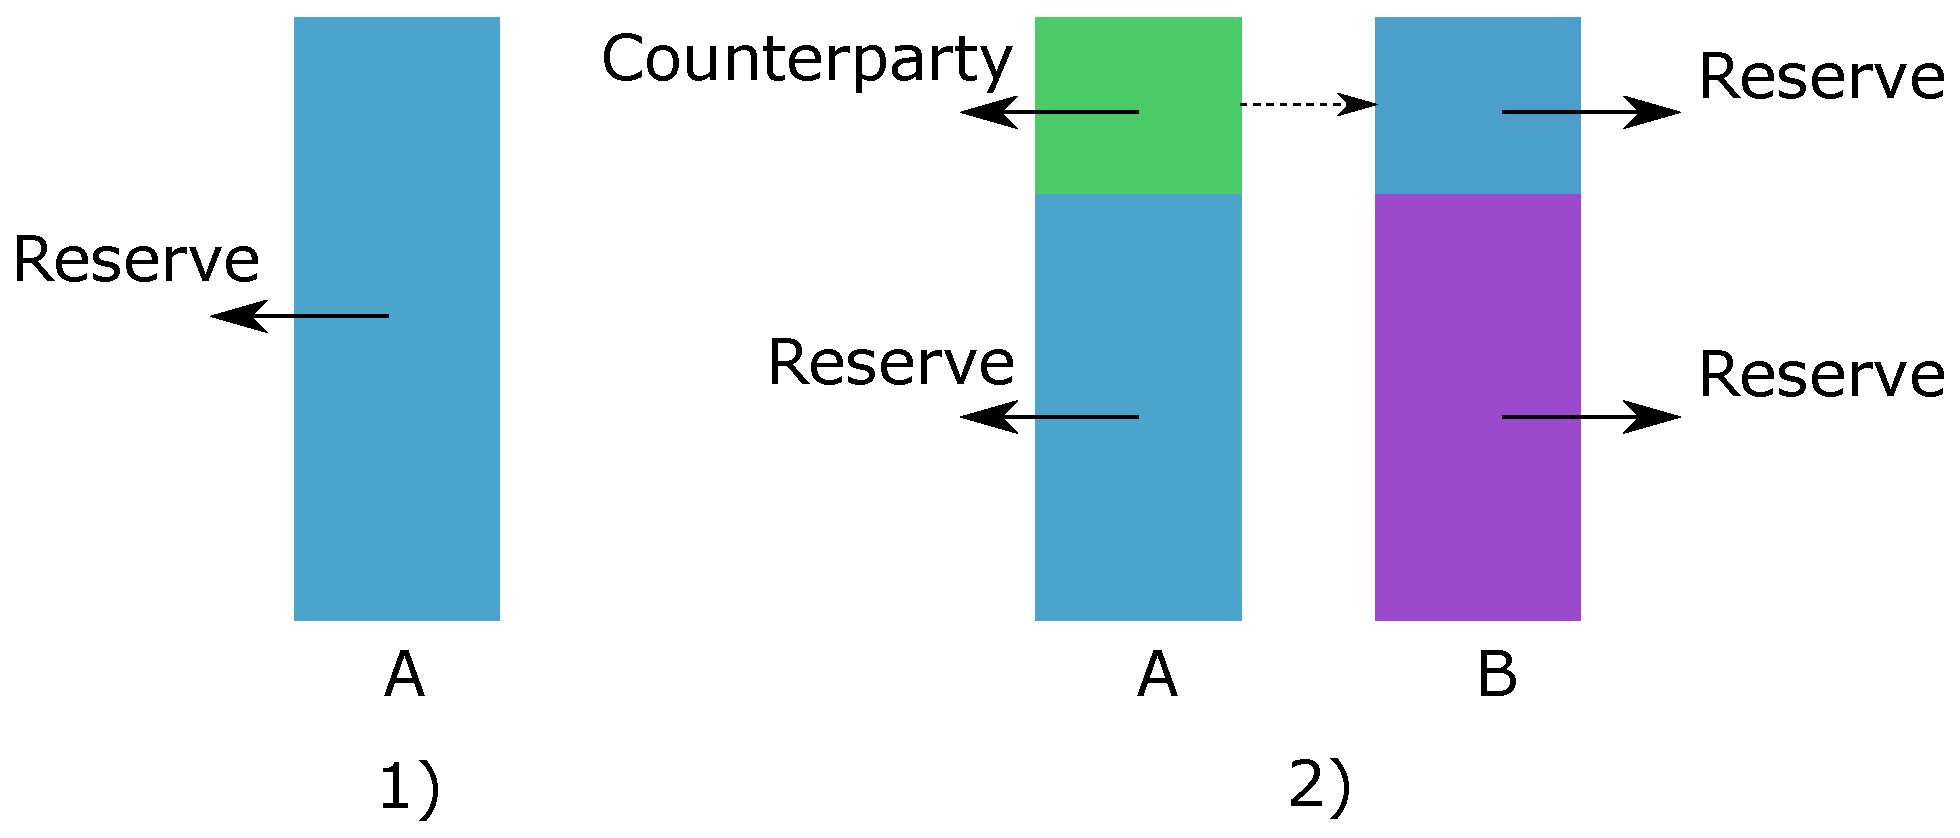
\includegraphics[width=\linewidth]{images/part1/reserve_vs_couterparty.eps}
  \caption{Comparison between reserve and counterparty risk. In case 1), the company hold all the risk, and this value is used to compute the reserve risk. In case 2), company A transferred a part of its risk to company B. The remaining share is used to compute reserve risk, whereas the transferred part (called recoverable) is used to compute a counterparty risk. Company B just add to its reserve risk the share received from A.}
  \label{fig:RESVSCOUNTER}
\end{figure}

The additional credit risk sub-capital $\Delta C_{cred}$ is computed by multiplying the additional recoverables $\Delta Recov$ by a factor $F_{cred}$ depending on the counterparty rating. 

\begin{equation}
	\Delta C_{cred} = \Delta Recov \; \times F_{cred}
\end{equation}

with $\Delta Recov$ the additional recoverables and $F_{cred}$ the credit risk factor.

The dependency of the factor toward the counterparty rating is presented in table \ref{t:BMA_CREDIT_FACTOR}

\begin{table}[h!]
\centering
\begin{tabular}{|l|l|l|}
\hline
   \textbf{BMA Rating} & \textbf{S \& P rating} & \textbf{Credit Factor F{cred} (\%)}  \\ \hline \hline
   0 & AA government & 0 \\ \hline
   1 & AAA          & 0.7  \\ \hline
   2 & AA+ to AA-   & 1.5 \\ \hline
   3 & A+ to A-     & 3.5 \\ \hline
   4 & BBB+ to BBB- & 7  \\ \hline
   5 & BB+ to BB-   & 12  \\ \hline
   6 & B+ to B-     & 20  \\ \hline
   7 & CCC+ to CCC- & 27  \\ \hline
   8 &below CCC-    & 35  \\ \hline
   \label{t:BMA_CREDIT_FACTOR}
\end{tabular}
   \caption{BMA Credit Risk factor by counterparty rating.}
\end{table}


\subsubsection{Investment risk : Spread Risk}

A very classical investment of (re)insurance companies is government and corporate bonds. A bond is an instrument of indebtedness of the bond issuer to the holder. It can be viewed as a loan from the bond issuer to the holder. One key point is that a bond grants an ownership right (like equity) of the company to the holder : it is debt that a company has toward the holder. A bond can be modeled as a series of cash flows. First the holder bears a negative cash flow when it buys the bond to the government of company. After, the company pays coupon (or interest), which are computed as a percentage of the principal (the borrowed sum), over the duration of the bond. The principal is payed at bond maturity.

As bonds can be traded, the value of a bond depends on how much the market is willing to pays for it. When the bond is issued, the interest rate is set at, for example, 5\% of the principal (sum payed to purchase the bond, which is the capital invested to get a 5\% additional money). After, the bond can be traded on the market. The current yield of a bond is the effective annual interest rate, computed as the coupon value divided by the current market value of the bond. If its market value decreases, it's yield increases (as the coupon value is set at the issuance of the bond).

A bond can be characterized by its credit/yield spread. This is the difference of yield between a given bond and a risk-free bond (US government bond for example). This yield reflect the riskiness of the bond compared to a risk-free one : if the probability of default of the bond issuer is higher than a risk free one, the investor wants a premium for this default risk. The more risky a bond, the higher its yield spread. 

One risk is the decreases of bond value after an interest rate move. If bond spread increases, as its coupon value is set, it mean that its price (ie the value at which it can be sold) decreases. This is a bad news for the insurance company which count on the bonds to pay its claims and provide additional investment revenues. The risk driver generally chosen by the regulator is the amount of fixed income instrument hold by the company.

TODO : CALCUL ?

\subsubsection{Investment risk : Equity investment Risk}

The Equity investment risk is the risk of a deviation of the value of equity hold as an investment by the (re)insurance company. As public listed companies' stocks can be easily traded, an economic downturn, the mismanagement of a company or political troubles can lead to a decrease of stocks value. Therefore, the equity portfolio value of the (re)insurance company can fluctuate and undergo an important decrease. This is particularly true in the case of a financial crisis like the 2007/2008 one.

The risk driver generally chosen by the regulator is the amount of equity hold by the company.


TODO : CALCUL ?

\subsubsection{Investment risk : Other investment Risk}

The Other investments risk is the risk of a deviation of the value of other investments hold by the (re)insurance company. Other investments can be of numerous types, as explained in section \ref{sec:FINANCIAL_STATEMENT}. For each type of investment the drivers of value fluctuation must be understood and assessed independently.

The value of real estate investments can decrease in the case of a mortgage crisis for example. As people cannot repay their mortgages, they are forced to sell their houses at a discounted price, leading to a decrease of housing prices. 
Private equity value can decrease if the company's performance is under expectations and if it goes bankrupt.

The risk driver generally chosen by the regulator is the amount of each investments hold (property, private equity, etc) by the company.

TODO : CALCUL OU NEGLIGEABLE ?

\subsubsection{Concentration risks}

The concentration risk represent the risk of aggregation of losses on assets that share common characteristics. For example, holding equity from only one company, operating on one business and in one country is a situation of high concentration risk. A way to decrease this risk is to invest in diversified companies, from a geographic and business line point of view.

